\documentclass{beamer}
% =============================================================================
% ENCODING
% =============================================================================
\usepackage[utf8]{inputenc}  % UTF-8 encoding support

% =============================================================================
% GRAPHICS
% =============================================================================
\usepackage{graphicx}  % For \includegraphics (401 uses across lectures)

% =============================================================================
% MATH PACKAGES
% =============================================================================
\usepackage{amsmath}    % For align, multline, equation environments (heavily used)
\usepackage{amsfonts}   % For \mathbb (e.g., \bbR, \bbE)
\usepackage{amssymb}    % For additional math symbols

% =============================================================================
% TABLES
% =============================================================================
\usepackage{booktabs}   % For \toprule, \midrule, \bottomrule (used in lecture13, lecture14)

% =============================================================================
% LISTS
% =============================================================================
\usepackage{enumerate}  % Enhanced enumerate environment (76 uses across lectures)

% =============================================================================
% TIKZ (DIAGRAMS)
% =============================================================================
\usepackage{tikz}       % For taxonomy diagram and footnotes positioning

% =============================================================================
% UTILITY PACKAGES
% =============================================================================
\usepackage{multido}    % For \multido command used in \eqpause
\usepackage{etoolbox}   % For \AtEndEnvironment, \ifbool, \newbool (used in preamble and taxonomy)
\usepackage{xspace}     % For smart spacing after custom commands (\ODESolve, \SDESolve)

% =============================================================================
% BEAMER THEME SETTINGS
% =============================================================================
\usetheme{default}
\usecolortheme{default}

\setbeamerfont{title}{size=\Huge}
\setbeamertemplate{footline}[frame number]{}
\setbeamertemplate{section in toc}[sections numbered]

\makeatletter
\newcommand\HUGE{\@setfontsize\Huge{35}{40}}
\makeatother    

\setbeamerfont{title}{size=\HUGE}
\beamertemplatenavigationsymbolsempty

% =============================================================================
% TIKZ LIBRARIES
% =============================================================================
% Used for taxonomy diagram: arrows, positioning, shapes
\usetikzlibrary{arrows.meta,calc,shapes,positioning,shadows,trees}

% =============================================================================
% CUSTOM FOOTNOTE COMMANDS
% =============================================================================
% \myfootnote{text} - creates a footnote at the bottom of the slide
\newcommand\myfootnote[1]{%
  \vspace{-0.5cm}%
  \tikz[remember picture,overlay]
  \draw (current page.south west) +(1in + \oddsidemargin,0.5em)
  node[anchor=south west,inner sep=0pt]{\parbox{\textwidth}{%
      \rlap{\rule{10em}{0.4pt}}\raggedright\scriptsize \textit{#1}}};}

% \myfootnotewithlink{url}{text} - creates a clickable footnote (623 uses across lectures)
\newcommand\myfootnotewithlink[2]{%
  \vspace{-0.5cm}%
  \tikz[remember picture,overlay]
  \draw (current page.south west) +(1in + \oddsidemargin,0.5em)
  node[anchor=south west,inner sep=0pt]{\parbox{\textwidth}{%
      \rlap{\rule{10em}{0.4pt}}\raggedright\scriptsize\href{#1}{\textit{#2}}}};}

% =============================================================================
% SECTION/SUBSECTION OUTLINE AUTOMATION
% =============================================================================
% Automatically show outline at the beginning of each section
\AtBeginSection[]
      {
      	\begin{frame}{Outline}
      		\tableofcontents[currentsection]
      	\end{frame}
      }
      \AtBeginSubsection[]{
      	\begin{frame}{Outline}
      		\tableofcontents[currentsection,currentsubsection]
      	\end{frame}
}

% =============================================================================
% CUSTOM SLIDE ANIMATION COMMANDS
% =============================================================================
% These commands enable step-by-step reveal of equations and content
% Used heavily across all lectures (1130+ uses of \nextonslide and \eqpause)

\newcounter{noscounter}   % Counter for \nextonslide (resets on each new slide)
\newcounter{pcounter}     % Counter for pause commands (resets after \eqpause)
\newcounter{diffcounter}  % Counts pauses after equations

% \nextonslide{content} - reveals content on the next overlay
\newcommand{\nextonslide}[1]{%
  \stepcounter{noscounter}%
  \stepcounter{pcounter}%
  \stepcounter{diffcounter}%
  \onslide<\value{noscounter}->{#1}%
}

% \resetonslide - resets all animation counters (called at each frame)
\newcommand{\resetonslide}{%
    \setcounter{noscounter}{1}%
    \setcounter{pcounter}{1}%
    \setcounter{diffcounter}{0}%
}

% \eqpause - pause after equation that syncs with \nextonslide
\newcommand{\eqpause}{%
  \multido{\i=1+1}{\value{pcounter}}{\pause}%
  \stepcounter{noscounter}%
  \setcounter{pcounter}{1}%
}

% \eqpausediff - helper command, runs automatically after math environments
\newcommand{\eqpausediff}{%
  \multido{\i=1+1}{\value{diffcounter}}{\pause}%
  \addtocounter{pcounter}{-\value{diffcounter}}%
  \setcounter{diffcounter}{0}%
}

% Apply \eqpausediff after math environments
\newcommand\AtEndBoth[2]{%
  \AtEndEnvironment{#1}{#2}%
  \AtEndEnvironment{#1*}{#2}%
}

\AtEndBoth{align}{\eqpausediff}
\AtEndBoth{equation}{\eqpausediff}
\AtEndBoth{multline}{\eqpausediff}

% Reset counters at the beginning of each frame
\addtobeamertemplate{frametitle}{\resetonslide}{}

% =============================================================================
% INCLUDE OTHER CONFIGURATION FILES
% =============================================================================
% ==============================================================================
% Custom LaTeX Commands for Deep Generative Models Course
% ==============================================================================

% ==============================================================================
% BOLD LETTERS (mathbf / boldsymbol)
% ==============================================================================

% ------------------------------------------------------------------------------
% Latin Bold Lowercase
% Usage: \bx for x in bold, commonly used for vectors
% ------------------------------------------------------------------------------
\newcommand{\ba}{\mathbf{a}}
\newcommand{\bc}{\mathbf{c}}
\newcommand{\be}{\mathbf{e}}
\newcommand{\bff}{\mathbf{f}}  % Note: \bf is reserved for bold font switching
\newcommand{\bg}{\mathbf{g}}
\newcommand{\bh}{\mathbf{h}}
\newcommand{\bp}{\mathbf{p}}
\newcommand{\bq}{\mathbf{q}}
\newcommand{\bs}{\mathbf{s}}
\newcommand{\bt}{\mathbf{t}}
\newcommand{\bu}{\mathbf{u}}
\newcommand{\bv}{\mathbf{v}}
\newcommand{\bw}{\mathbf{w}}
\newcommand{\bx}{\mathbf{x}}
\newcommand{\by}{\mathbf{y}}
\newcommand{\bz}{\mathbf{z}}
\newcommand{\bzero}{\boldsymbol{0}}  % Zero vector
\newcommand{\bone}{\mathbf{1}}       % Ones vector

% ------------------------------------------------------------------------------
% Latin Bold Uppercase
% Usage: \bX for X in bold, commonly used for matrices or random vectors
% ------------------------------------------------------------------------------
\newcommand{\bA}{\mathbf{A}}
\newcommand{\bG}{\mathbf{G}}
\newcommand{\bI}{\mathbf{I}}
\newcommand{\bJ}{\mathbf{J}}
\newcommand{\bL}{\mathbf{L}}
\newcommand{\bM}{\mathbf{M}}
\newcommand{\bP}{\mathbf{P}}
\newcommand{\bQ}{\mathbf{Q}}
\newcommand{\bR}{\mathbf{R}}
\newcommand{\bT}{\mathbf{T}}
\newcommand{\bU}{\mathbf{U}}
\newcommand{\bV}{\mathbf{V}}
\newcommand{\bW}{\mathbf{W}}
\newcommand{\bX}{\mathbf{X}}
\newcommand{\bZ}{\mathbf{Z}}

% ------------------------------------------------------------------------------
% Greek Bold Lowercase
% Usage: \btheta for θ in bold, commonly used for parameter vectors
% ------------------------------------------------------------------------------
\newcommand{\bepsilon}{\boldsymbol{\epsilon}}
\newcommand{\blambda}{\boldsymbol{\lambda}}
\newcommand{\bmu}{\boldsymbol{\mu}}
\newcommand{\bphi}{\boldsymbol{\phi}}
\newcommand{\bpi}{\boldsymbol{\pi}}
\newcommand{\bpsi}{\boldsymbol{\psi}}
\newcommand{\bsigma}{\boldsymbol{\sigma}}
\newcommand{\btheta}{\boldsymbol{\theta}}

% ------------------------------------------------------------------------------
% Greek Bold Uppercase
% Usage: \bSigma for Σ in bold, commonly used for covariance matrices
% ------------------------------------------------------------------------------
\newcommand{\bPhi}{\boldsymbol{\Phi}}
\newcommand{\bSigma}{\boldsymbol{\Sigma}}
\newcommand{\bTheta}{\boldsymbol{\Theta}}

% ==============================================================================
% CALLIGRAPHIC LETTERS (mathcal)
% Usage: \cX for calligraphic X, commonly used for sets and spaces
% ==============================================================================
\newcommand{\cF}{\mathcal{F}}
\newcommand{\cI}{\mathcal{I}}
\newcommand{\cL}{\mathcal{L}}
\newcommand{\cM}{\mathcal{M}}
\newcommand{\cN}{\mathcal{N}}
\newcommand{\cO}{\mathcal{O}}
\newcommand{\cP}{\mathcal{P}}
\newcommand{\cS}{\mathcal{S}}
\newcommand{\cT}{\mathcal{T}}
\newcommand{\cW}{\mathcal{W}}
\newcommand{\cX}{\mathcal{X}}
\newcommand{\cZ}{\mathcal{Z}}

% ==============================================================================
% BLACKBOARD BOLD LETTERS (mathbb)
% Usage: \bbR for ℝ, commonly used for number sets and expectations
% ==============================================================================
\newcommand{\bbE}{\mathbb{E}}  % Expectation
\newcommand{\bbI}{\mathbb{I}}  % Indicator function
\newcommand{\bbP}{\mathbb{P}}  % Probability measure
\newcommand{\bbR}{\mathbb{R}}  % Real numbers

% ==============================================================================
% MATH OPERATORS
% ==============================================================================

% ------------------------------------------------------------------------------
% Optimization Operators
% Usage: \argmin_{x} f(x) for proper spacing and limits placement
% ------------------------------------------------------------------------------
\DeclareMathOperator*{\argmin}{arg\,min}
\DeclareMathOperator*{\argmax}{arg\,max}

% ------------------------------------------------------------------------------
% Statistical Operators
% Usage: \cov(X, Y) for covariance
% ------------------------------------------------------------------------------
\DeclareMathOperator{\cov}{cov}

% ------------------------------------------------------------------------------
% Linear Algebra Operators
% Usage: \tr(\bA) for trace of matrix A
% ------------------------------------------------------------------------------
\DeclareMathOperator{\tr}{tr}

% ------------------------------------------------------------------------------
% Other Mathematical Operators
% ------------------------------------------------------------------------------
\DeclareMathOperator{\diver}{div}      % Divergence (vector calculus)
\newcommand{\sg}{\mathrm{sg}}          % Stop-gradient operator
\DeclareMathOperator{\softmax}{softmax}
\DeclareMathOperator{\supp}{supp}      % Support of a distribution

% ==============================================================================
% PROBABILITY DISTRIBUTIONS
% Usage: X \sim \cN(0, 1), Y \sim \Bern(p)
% ==============================================================================
\DeclareMathOperator{\Bern}{Bern}      % Bernoulli distribution
\DeclareMathOperator{\Cat}{Cat}        % Categorical distribution
\DeclareMathOperator{\Gumbel}{Gumbel}  % Gumbel distribution
\DeclareMathOperator{\Uniform}{Uniform}

% ==============================================================================
% METRICS AND DIVERGENCES
% Usage: \KL(p \| q), \JSD(p, q)
% ==============================================================================
\newcommand{\Ent}{\mathrm{H}}          % Entropy
\newcommand{\FID}{\mathrm{FID}}        % Fréchet Inception Distance
\newcommand{\JSD}{D_\mathrm{JS}}        % Jensen-Shannon Divergence
\newcommand{\KL}{D_\mathrm{KL}}        % Kullback-Leibler Divergence
\DeclareMathOperator{\MMD}{MMD}        % Maximum Mean Discrepancy
\DeclareMathOperator{\SNR}{SNR}        % Signal-to-Noise Ratio

% ==============================================================================
% NEURAL NETWORK NOTATION
% ==============================================================================

% ------------------------------------------------------------------------------
% Network Architectures (upright font for abbreviations)
% Usage: f_{\btheta} = \NN_{\btheta}(\bx)
% ------------------------------------------------------------------------------
\newcommand{\MLP}{\mathrm{MLP}}        % Multi-Layer Perceptron
\newcommand{\NN}{\mathrm{NN}}          % Neural Network
\newcommand{\RNN}{\mathrm{RNN}}        % Recurrent Neural Network

% ------------------------------------------------------------------------------
% Numerical Solvers (monospace font)
% Usage: \bx_T = \ODESolve(v, \bx_0, T)
% ------------------------------------------------------------------------------
\newcommand{\ODESolve}{\texttt{ODESolve}\xspace}
\newcommand{\SDESolve}{\texttt{SDESolve}\xspace}

% ==============================================================================
% COMMON SHORTCUTS
% Usage: Frequently used subscripted or parameterized expressions
% ==============================================================================
\newcommand{\pd}{p_{\text{data}}}              % Data distribution
\newcommand{\pt}{p_{\boldsymbol{\theta}}}      % Parameterized distribution
\newcommand{\qagg}{q_{\text{agg}}}             % Aggregated posterior
\newcommand{\lambdamax}{\lambda_{\text{max}}}  % Maximum eigenvalue
  % Math shorthand commands (\bx, \bbE, \KL, etc.)
\input{../utils/title}        % Title page template
% For each possible node, we create a boolean
\newbool{hl@root}
\newbool{hl@explicit}
\newbool{hl@implicit}
\newbool{hl@exact}
\newbool{hl@approx}
\newbool{hl@gan}
\newbool{hl@ar}
\newbool{hl@nf}
\newbool{hl@vae}
\newbool{hl@score}
\newbool{hl@cont}
\newbool{hl@ddpm}
\newbool{hl@sm}
\newbool{hl@ode}
\newbool{hl@sde}
\newbool{hl@fm}

% Command to reset all bools
\newcommand{\resetAllHighlights}{%
    \boolfalse{hl@root}%
    \boolfalse{hl@explicit}%
    \boolfalse{hl@implicit}%
    \boolfalse{hl@exact}%
    \boolfalse{hl@approx}%
    \boolfalse{hl@gan}%
    \boolfalse{hl@ar}%
    \boolfalse{hl@nf}%
    \boolfalse{hl@vae}%
    \boolfalse{hl@score}%
    \boolfalse{hl@cont}%
    \boolfalse{hl@ddpm}%
    \boolfalse{hl@sm}%
    \boolfalse{hl@ode}%
    \boolfalse{hl@sde}%
    \boolfalse{hl@fm}%
}

% Command to set a single highlight
\newcommand{\setHighlight}[1]{%
    \booltrue{hl@#1}%
}

% Command to set highlights from comma-separated list
\newcommand{\setHighlights}[1]{%
    \resetAllHighlights%
    \forcsvlist{\setHighlight}{#1}%
}

% Highlighted style definition
\tikzset{
    hl/.style={line width=1.2pt, draw=black, font=\scriptsize\bfseries},
    box/.style={
        rectangle, 
        draw=gray!50, 
        rounded corners=2pt, 
        minimum width=1.9cm, 
        minimum height=0.5cm, 
        align=center, 
        font=\scriptsize, 
        line width=0.4pt
    },
    rootnode/.style={box, fill=violet!20},
    category/.style={box, fill=teal!20},
    model/.style={box, fill=yellow!30},
    arrow/.style={-Stealth, draw=gray!80, line width=0.4pt}
}

% Draw taxonomy with pre-set highlights
\newcommand{\drawTaxonomy}{%
    \begin{tikzpicture}[scale=0.9, transform shape, node distance=0.6cm and 0.3cm]
        % --- CENTRAL ROOT ---
        \ifbool{hl@root}{\node[rootnode, hl] (root) {Generative Models};}{\node[rootnode] (root) {Generative Models};}

        % --- UPPER BRANCHES ---
        \ifbool{hl@explicit}{\node[category, hl, above left=0.6cm and 0.5cm of root] (explicit) {Explicit density};}{\node[category, above left=0.6cm and 0.5cm of root] (explicit) {Explicit density};}
        \ifbool{hl@implicit}{\node[category, hl, above right=0.6cm and 0.5cm of root] (implicit) {Implicit density};}{\node[category, above right=0.6cm and 0.5cm of root] (implicit) {Implicit density};}

        \ifbool{hl@exact}{\node[category, hl, above left=0.6cm and -0.6cm of explicit] (exact) {Exact likelihood};}{\node[category, above left=0.6cm and -0.6cm of explicit] (exact) {Exact likelihood};}
        \ifbool{hl@approx}{\node[category, hl, above right=0.6cm and -0.6cm of explicit] (approx) {Approximate likelihood};}{\node[category, above right=0.6cm and -0.6cm of explicit] (approx) {Approximate likelihood};}

        \ifbool{hl@gan}{\node[model, hl, above=0.6cm of implicit] (gans) {GANs};}{\node[model, above=0.6cm of implicit] (gans) {GANs};}

        \ifbool{hl@ar}{\node[model, hl, above left=0.6cm and -0.9cm of exact] (ar) {Autoregressive \\ models};}{\node[model, above left=0.6cm and -0.9cm of exact] (ar) {Autoregressive \\ models};}
        \ifbool{hl@nf}{\node[model, hl, above right=0.6cm and -0.9cm of exact] (nf) {Normalizing \\ Flows};}{\node[model, above right=0.6cm and -0.9cm of exact] (nf) {Normalizing \\ Flows};}
        \ifbool{hl@vae}{\node[model, hl, above=0.6cm of approx] (vae) {Variational \\ Autoencoders};}{\node[model, above=0.6cm of approx] (vae) {Variational \\ Autoencoders};}

        % --- LOWER BRANCHES ---
        \ifbool{hl@score}{\node[category, hl, below left=0.6cm and 0.5cm of root] (score) {Score-based};}{\node[category, below left=0.6cm and 0.5cm of root] (score) {Score-based};}
        \ifbool{hl@cont}{\node[category, hl, below right=0.6cm and 0.5cm of root] (cont) {Continuous \\ dynamics};}{\node[category, below right=0.6cm and 0.5cm of root] (cont) {Continuous \\ dynamics};}

        \ifbool{hl@sm}{\node[model, hl, below left=0.6cm and -0.8cm of score] (sm) {Score Matching};}{\node[model, below left=0.6cm and -0.8cm of score] (sm) {Score Matching};}
        \ifbool{hl@ddpm}{\node[model, hl, below right=0.6cm and -0.8cm of score] (ddpm) {Denoising Diffusion};}{\node[model, below right=0.6cm and -0.8cm of score] (ddpm) {Denoising Diffusion};}

        \ifbool{hl@ode}{\node[model, hl, below left=0.6cm and -0.8cm of cont] (ode) {Neural ODEs};}{\node[model, below left=0.6cm and -0.8cm of cont] (ode) {Neural ODEs};}
        \ifbool{hl@sde}{\node[model, hl, below right=0.6cm and -0.8cm of cont] (sde) {SDE-based \\ Diffusion};}{\node[model, below right=0.6cm and -0.8cm of cont] (sde) {SDE-based \\ Diffusion};}

        \ifbool{hl@fm}{\node[model, hl, below=0.6cm of ode] (fm) {Flow Matching};}{\node[model, below=0.6cm of ode] (fm) {Flow Matching};}

        % --- CONNECTIONS ---
        \draw[arrow] (root.north) -- ++(0,0.3) -| (explicit.south);
        \draw[arrow] (root.north) -- ++(0,0.3) -| (implicit.south);
        \draw[arrow] (root.south) -- ++(0,-0.3) -| (score.north);
        \draw[arrow] (root.south) -- ++(0,-0.3) -| (cont.north);
        \draw[arrow] (explicit.north) -- ++(0,0.3) -| (exact.south);
        \draw[arrow] (explicit.north) -- ++(0,0.3) -| (approx.south);
        \draw[arrow] (exact.north) -- ++(0,0.3) -| (ar.south);
        \draw[arrow] (exact.north) -- ++(0,0.3) -| (nf.south);
        \draw[arrow] (approx.north) -- (vae.south);
        \draw[arrow] (implicit.north) -- (gans.south);
        \draw[arrow] (score.south) -- ++(0,-0.3) -| (sm.north);
        \draw[arrow] (score.south) -- ++(0,-0.3) -| (ddpm.north);
        \draw[arrow] (cont.south) -- ++(0,-0.3) -| (ode.north);
        \draw[arrow] (cont.south) -- ++(0,-0.3) -| (sde.north);
        \draw[arrow] (ode.south) -- (fm.north);
    \end{tikzpicture}
}

% The main taxonomy rendering command
\newcommand{\renderTaxonomy}[1]{%
    \setHighlights{#1}%
    \centering
    \drawTaxonomy%
}     % Generative models taxonomy diagram

\createdgmtitle{9}
%--------------------------------------------------------------------------------
\begin{document}
%--------------------------------------------------------------------------------
\begin{frame}[noframenumbering,plain]
\titlepage
    \resetonslide
\end{frame}
%=======
\begin{frame}{Recap of Previous Lecture}
	\myfootnotewithlink{https://arxiv.org/abs/2006.11239}{Ho J. Denoising Diffusion Probabilistic Models, 2020}
	\begin{block}{ELBO for Gaussian Diffusion Model}
		\vspace{-0.7cm}
		\begin{multline*}
			\cL_{\bphi, \btheta}(\bx) =  {\color{olive}\bbE_{q(\bx_1 | \bx_0)} \log \pt(\bx_0 | \bx_1)} - {\color{violet}\KL\bigl(q(\bx_T | \bx_0) \| p(\bx_T)\bigr)} - \\
			- \sum_{t=2}^T  \underbrace{ \bbE_{q(\bx_t | \bx_0)}\KL \bigl(q(\bx_{t-1} | \bx_t, \bx_0) \| \pt(\bx_{t-1} | \bx_t)\bigr)}_{\cL_t}
		\end{multline*}
		\vspace{-1.0cm}
	\end{block}
	\begin{align*}
		q(\bx_{t-1} | \bx_t, \bx_0) &= \cN(\bx_{t-1} | \tilde{\bmu}_t(\bx_t, \bx_0), \tilde{\beta}_t \bI), \\
		\pt(\bx_{t - 1} | \bx_t) &= \cN \bigl(\bx_{t - 1} | \bmu_{\btheta, t}(\bx_t), {\color{violet}\bsigma_{\btheta, t}^2(\bx_t)}\bigr)
	\end{align*}
	It is assumed that ${\color{violet}\bsigma_{\btheta, t}^2(\bx_t) = \tilde{\beta}_t \bI}$.
	\[
		\cL_t = \bbE_{q(\bx_t | \bx_0)} \left[\frac{1}{2\tilde{\beta}_t} \bigl\| \tilde{\bmu}_t(\bx_t, \bx_0) - \bmu_{\btheta, t}(\bx_t) \bigr\|^2  \right]
	\]
\end{frame}
%=======
\begin{frame}{Recap of Previous Lecture}
	\myfootnotewithlink{https://arxiv.org/abs/2006.11239}{Ho J. Denoising Diffusion Probabilistic Models, 2020}
	\[
		\cL_t = \bbE_{\color{violet}q(\bx_t | \bx_0)} \left[ {\color{olive}\frac{1}{2\tilde{\beta}_t}} \bigl\| \tilde{\bmu}_t(\bx_t, \bx_0) - \bmu_{\btheta, t}(\bx_t) \bigr\|^2  \right]
	\]
	\vspace{-0.3cm}
	\begin{block}{Reparametrization}
		\vspace{-0.7cm}
		\begin{align*}
			\tilde{\bmu}_t(\bx_t, \bx_0) &= \frac{1}{\sqrt{\alpha_t}} \cdot \bx_t - \frac{1 - \alpha_t}{\sqrt{\alpha_t (1 - \bar{\alpha}_t)}} \cdot \bepsilon \\
			\bmu_{\btheta, t}(\bx_t) &= \frac{1}{\sqrt{\alpha_t}} \cdot \bx_t - {\color{teal}\frac{1 - \alpha_t}{\sqrt{\alpha_t (1 - \bar{\alpha}_t)}}} \cdot \bepsilon_{\btheta, t}(\bx_t)
		\end{align*}
		\vspace{-0.7cm}
	\end{block}
	\vspace{-0.2cm}
	\[
		\cL_t  =	 \bbE_{\color{violet}\bepsilon \sim \cN(0, \bI)} \left[ \frac{(1 - \alpha_t)^2}{2\tilde{\beta}_t \alpha_t (1 - \bar{\alpha}_t)} \Bigl\| \bepsilon - \bepsilon_{\btheta, t}\bigl( {\color{teal}\sqrt{\bar{\alpha}_t} \bx_0 + \sqrt{1 - \bar{\alpha}_t} \bepsilon}\bigr) \Bigr\|^2 \right]
	\]
	At every step of the reverse process, we attempt to predict the noise~$\bepsilon$ that was used in the forward diffusion process!
	\begin{block}{Simplified Objective}
		\vspace{-0.7cm}
		\[
			 \cL_{\text{simple}} = \bbE_{t \sim U\{1, T\}} \bbE_{\bepsilon \sim \cN(0, \bI)} \Bigl\| \bepsilon - \bepsilon_{\btheta, t}\bigl( \sqrt{\bar{\alpha}_t} \cdot \bx_0 + \sqrt{1 - \bar{\alpha}_t} \cdot \bepsilon\bigr) \Bigr\|^2
		\]
	\end{block}
\end{frame}
%=======
\begin{frame}{Recap of Previous Lecture}
	\myfootnotewithlink{https://arxiv.org/abs/2006.11239}{Ho J. Denoising Diffusion Probabilistic Models, 2020}
	\begin{block}{Training}
		\begin{enumerate}
			\item Sample $\bx_0 \sim \pd(\bx)$, $t \sim U\{1, T\}$, $\bepsilon \sim \cN(0, \bI)$.
			\item Compute noisy image $\bx_t = \sqrt{\bar{\alpha}_t} \cdot \bx_0 + \sqrt{1 - \bar{\alpha}_t} \cdot \bepsilon$.
			\item Compute loss $ \cL_{\text{simple}} = \| \bepsilon - \bepsilon_{\btheta, t}(\bx_t) \|^2 $.
		\end{enumerate}
	\end{block}
	\begin{block}{Sampling (Ancestral)}
		\begin{enumerate}
			\item Sample $\bx_T \sim \cN(0, \bI)$.
			\item Compute the mean of $\pt(\bx_{t-1} | \bx_t) = \cN(\bmu_{\btheta, t}(\bx_t), \tilde{\beta}_t \cdot \bI)$:
			\vspace{-0.3cm}
			\[
				\bmu_{\btheta, t}(\bx_t) = \frac{1}{\sqrt{\alpha_t}} \cdot \bx_t - \frac{1 - \alpha_t}{\sqrt{\alpha_t (1 - \bar{\alpha}_t)}} \cdot \bepsilon_{\btheta, t}(\bx_t).
			\]
			\vspace{-0.5cm}
			\item Denoise $\bx_{t - 1} = \bmu_{\btheta, t}(\bx_t) +  \sqrt{\tilde{\beta}_t} \cdot \bepsilon$, $\bepsilon \sim \cN(0, \bI)$.
		\end{enumerate}
	\end{block}
\end{frame}
%=======
\begin{frame}{Recap of Previous Lecture}
	\myfootnotewithlink{https://arxiv.org/abs/2006.11239}{Ho J. Denoising Diffusion Probabilistic Models, 2020}
	\begin{block}{DDPM Objective}
		\vspace{-0.5cm}
		\[
			\bbE_{\pd(\bx_0)} \bbE_{t \sim U\{1, T\}}\bbE_{q(\bx_t | \bx_0)} \left[ {\color{olive}C_{2, t}} \Bigl\|  \bs_{\btheta, t} (\bx_t) - \nabla_{\bx_t} \log q(\bx_t | \bx_0) \Bigr\|_2^2  \right]
		\]
		\[
			\bx_t = \sqrt{\bar{\alpha}_t} \cdot \bx_0 + \sqrt{1 - \bar{\alpha}_t} \cdot \bepsilon
		\]
		In practice, {\color{olive}this coefficient} is often omitted.
	\end{block}
	\begin{block}{NCSN Objective}
		\vspace{-0.3cm}
		\[
			\bbE_{\pd(\bx_0)} \bbE_{t \sim U\{1, T\}} \bbE_{q(\bx_t | \bx_0)}\bigl\| \bs_{\btheta, \sigma_t}(\bx_t) - \nabla_{\bx_t} \log q(\bx_t | \bx_0) \bigr\|^2_2 
		\]
		\vspace{-0.3cm}
	\end{block}
	\textbf{Note:} The objectives of DDPM and NCSN are almost identical; however, their sampling procedures differ:
	\begin{itemize}
		\item NCSN utilizes annealed Langevin dynamics,
		\item DDPM employs ancestral sampling.
	\end{itemize}
\end{frame}
%=======
\begin{frame}{Recap of Previous Lecture}
	\myfootnote{\href{https://arxiv.org/abs/2107.00630}{Kingma D. et al. Variational Diffusion Models, 2021} \\
	\href{https://arxiv.org/abs/2011.13456}{Song Y. et al. Score-Based Generative Modeling through Stochastic Differential Equations, 2020}}
	\begin{block}{Summary}
		\begin{itemize}
		\item Different Markov chains:
			\begin{itemize}
				\item DDPM: $\bx_t = \sqrt{\bar{\alpha}_t} \cdot \bx_0 + \sqrt{1 - \bar{\alpha}_t} \cdot \bepsilon$;
				\item NCSN: $\bx_t = \bx_0 + \sigma_t \cdot \bepsilon$.
				\item One can generalize to $q(\bx_t |\bx_0) = \cN(\alpha_t \cdot \bx_0, \sigma^2_t\, \bI)$.
			\end{itemize}
		\eqpause
		\item The objectives coincide: ELBO $\equiv$ score-matching.
		\eqpause
		\item The sampling procedures differ:
			\begin{itemize}
				\item Ancestral sampling in DDPM;
				\item Annealed Langevin dynamics for NCSN;
				\item Hybrid approaches that combine both updates are possible.
			\end{itemize}
		\end{itemize}
	\end{block}
\end{frame}
%=======
\begin{frame}{Recap of Previous Lecture}
	\myfootnotewithlink{https://arxiv.org/abs/2105.05233}{Dhariwal P., Nichol A. Diffusion Models Beat GANs on Image Synthesis, 2021}
	\begin{block}{DDPM Sampling}
		\vspace{-0.3cm}
		\[
			\bx_{t - 1} = \frac{1}{\sqrt{1 - \beta_t}} \cdot \bx_t + \frac{\beta_t}{\sqrt{1 - \beta_t}} \cdot {\color{teal} \nabla_{\bx_t} \log \pt(\bx_t)} +  \sigma_t \cdot \bepsilon
		\]
		\vspace{-0.5cm}
	\end{block}
	\begin{block}{Guided Generation}
		\vspace{-0.5cm}
		\[
			\bx_{t - 1} =  \frac{1}{\sqrt{1 - \beta_t}}\cdot \bx_t +  \frac{\beta_t}{\sqrt{1 - \beta_t}}  \cdot  \nabla_{\bx_t} \log \pt(\bx_t | {\color{olive}\by}) +  \sigma_t \cdot \bepsilon
		\]
		\vspace{-0.5cm}
	\end{block}
	\begin{block}{Guided Generation}
		\vspace{-0.5cm}
		\begin{align*}
			{\color{olive}\nabla_{\bx_t} \log \pt(\bx_t | \by)} &
			= {\color{violet}\nabla_{\bx_t} \log \pt(\bx_t)} + \nabla_{\bx_t} \log p(\by | \bx_t) \\
			&= {\color{violet} \bs_{\btheta, t}(\bx_t)} + {\color{teal}\nabla_{\bx_t} \log p(\by | \bx_t)}
		\end{align*}
		\vspace{-0.5cm}
	\end{block}
	Here, $p(\by | \bx_t)$ denotes a classifier operating on noisy samples (which must be trained separately).
\end{frame}
%=======
\begin{frame}{Recap of Previous Lecture}
	\myfootnotewithlink{https://arxiv.org/abs/2105.05233}{Dhariwal P., Nichol A. Diffusion Models Beat GANs on Image Synthesis, 2021}
	\begin{block}{Guided Score Function}
		\vspace{-0.5cm}
		\begin{align*}
			\bs_{\btheta, t}(\bx_t, \by) &= \bs_{\btheta, t}(\bx_t) + \nabla_{\bx_t} \log p(\by | \bx_t) \\
			{\color{violet}\bs^{\gamma}_{\btheta, t}(\bx_t, \by)} &= \bs_{\btheta, t}(\bx_t) + {\color{teal}\gamma} \cdot \nabla_{\bx_t} \log p(\by | \bx_t)
		\end{align*}
		\vspace{-0.5cm}
	\end{block}
	\textbf{Note:} Increasing $\gamma$ sharpens $p(\by | \bx_t)$, increasing the contrast
	\[
		\hat{p}(\by | \bx_t) \propto p(\by | \bx_t)^{\gamma}.
	\]
	\vspace{-1.0cm}
	\begin{block}{Training}
		\begin{enumerate}
			\item Train the DDPM as before.
			\item Train an additional classifier $p(\by | \bx_t)$ on noisy data (time-dependent).
		\end{enumerate}
		\vspace{-0.5cm}
	\end{block}
	\vspace{-0.2cm}
	\begin{block}{Sampling (Guided)}
		\begin{enumerate}
			\item Sample $\bx_T \sim \cN(0, \bI)$.
			\item Denoise with the scaled guided score function:
			\vspace{-0.3cm}
			\[
				\bx_{t-1} = \frac{1}{\sqrt{1 - \beta_t}} \cdot \bx_t + \frac{\beta_t}{\sqrt{1 - \beta_t}} \cdot  {\color{olive}\bs^{\gamma}_{\btheta, t}(\bx_t, \by)} + \sigma_t \cdot \bepsilon.
			\]
			\vspace{-0.5cm}
		\end{enumerate}
	\end{block}
\end{frame}
%=======
\begin{frame}{Recap of Previous Lecture}
	\myfootnote{\href{https://arxiv.org/abs/2207.12598}{Ho J., Salimans T. Classifier-Free Diffusion Guidance, 2022} \\
	\href{https://arxiv.org/abs/2506.02070}{Holderrieth P., Erives E. An Introduction to Flow Matching and Diffusion Models, 2025}}
	The previous method requires an additional classifier $p(\by | \bx_t)$ trained on noisy data. Let's try to avoid this requirement.
	\[
		{\color{teal}\nabla_{\bx_t} \log p(\by | \bx_t)} =  \nabla_{\bx_t} \log \pt(\bx_t| \by) -\nabla_{\bx_t} \log  \pt(\bx_t)
	\]
	\vspace{-0.9cm}
	\begin{multline*}
		\nabla_{\bx_t}^{\gamma} \log \pt(\bx_t | \by) = \nabla_{\bx_t} \log \pt(\bx_t) + \gamma \cdot {\color{teal} \nabla_{\bx_t} \log p(\by | \bx_t)} = \\
		= \nabla_{\bx_t} \log \pt(\bx_t) + \gamma \cdot \bigl( {\color{teal}\nabla_{\bx_t} \log \pt(\bx_t| \by) - \nabla_{\bx_t} \log  \pt(\bx_t)} \bigr) = \\
		=  (1 - \gamma) \cdot  \nabla_{\bx_t} \log \pt(\bx_t) + \gamma \cdot  \nabla_{\bx_t} \log \pt(\bx_t| \by)
	\end{multline*}
	\vspace{-0.7cm}
	\begin{block}{Scaled Guided Score Function}
		\vspace{-0.3cm}
		\[
			\bs^{\gamma}_{\btheta, t}(\bx_t, \by) = (1 - \gamma) \cdot \bs_{\btheta, t}(\bx_t) +  \gamma \cdot \bs_{\btheta, t}(\bx_t, \by)
		\]
		\vspace{-0.5cm}
	\end{block}
	\vspace{-0.3cm}
	\begin{block}{CFG}
		\begin{enumerate}
			\item Introduce the ``absence of conditioning'' label $\by = \varnothing$.
			\item Identify the unguided score function $\bs_{\btheta, t}(\bx_t) = \bs_{\btheta, t}(\bx_t, \varnothing)$.
			\item Train a single model $\bs_{\btheta, t}(\bx_t, \by)$ on \textbf{supervised} data, dropping the label $\by$ with some fixed probability (simulating $\by = \varnothing$).
			\item At inference, evaluate the model twice to obtain $\bs_{\btheta, t}(\bx_t, \varnothing)$ and $\bs_{\btheta, t}(\bx_t, \by)$.
		\end{enumerate}
	\end{block}
\end{frame}
%=======
\begin{frame}{Outline}
	\tableofcontents
\end{frame}
%=======
\section{Continuous-Time Normalizing Flows (CNF)}
%=======
\begin{frame}{Discrete-Time Normalizing Flows}
	\myfootnotewithlink{https://lilianweng.github.io/lil-log/2018/10/13/flow-based-deep-generative-models.html}{https://lilianweng.github.io/lil-log/2018/10/13/flow-based-deep-generative-models.html}
	\vspace{-0.3cm}
	\begin{block}{Change of Variable Theorem (CoV)}
		Let $\bx$ be a random variable with density $p(\bx)$, and let $\bff: \bbR^m \rightarrow \bbR^m$ be a differentiable and \textbf{invertible} transformation. If $\bz = \bff(\bx)$, $\bx = \bff^{-1}(\bz) = \bg(\bz)$, then
		\vspace{-0.3cm}
		\[
			p(\bx) = p(\bz) |\det(\bJ_{\bff})| = p(\bz) \left|\det \left( \frac{\partial \bz}{\partial \bx} \right) \right| = p(\bff(\bx)) \left|\det \left(  \frac{\partial \bff(\bx)}{\partial \bx} \right) \right|
		\]
		\vspace{-0.5cm}
	\end{block}
	\eqpause

	\vspace{-0.3cm}
	\begin{figure}
		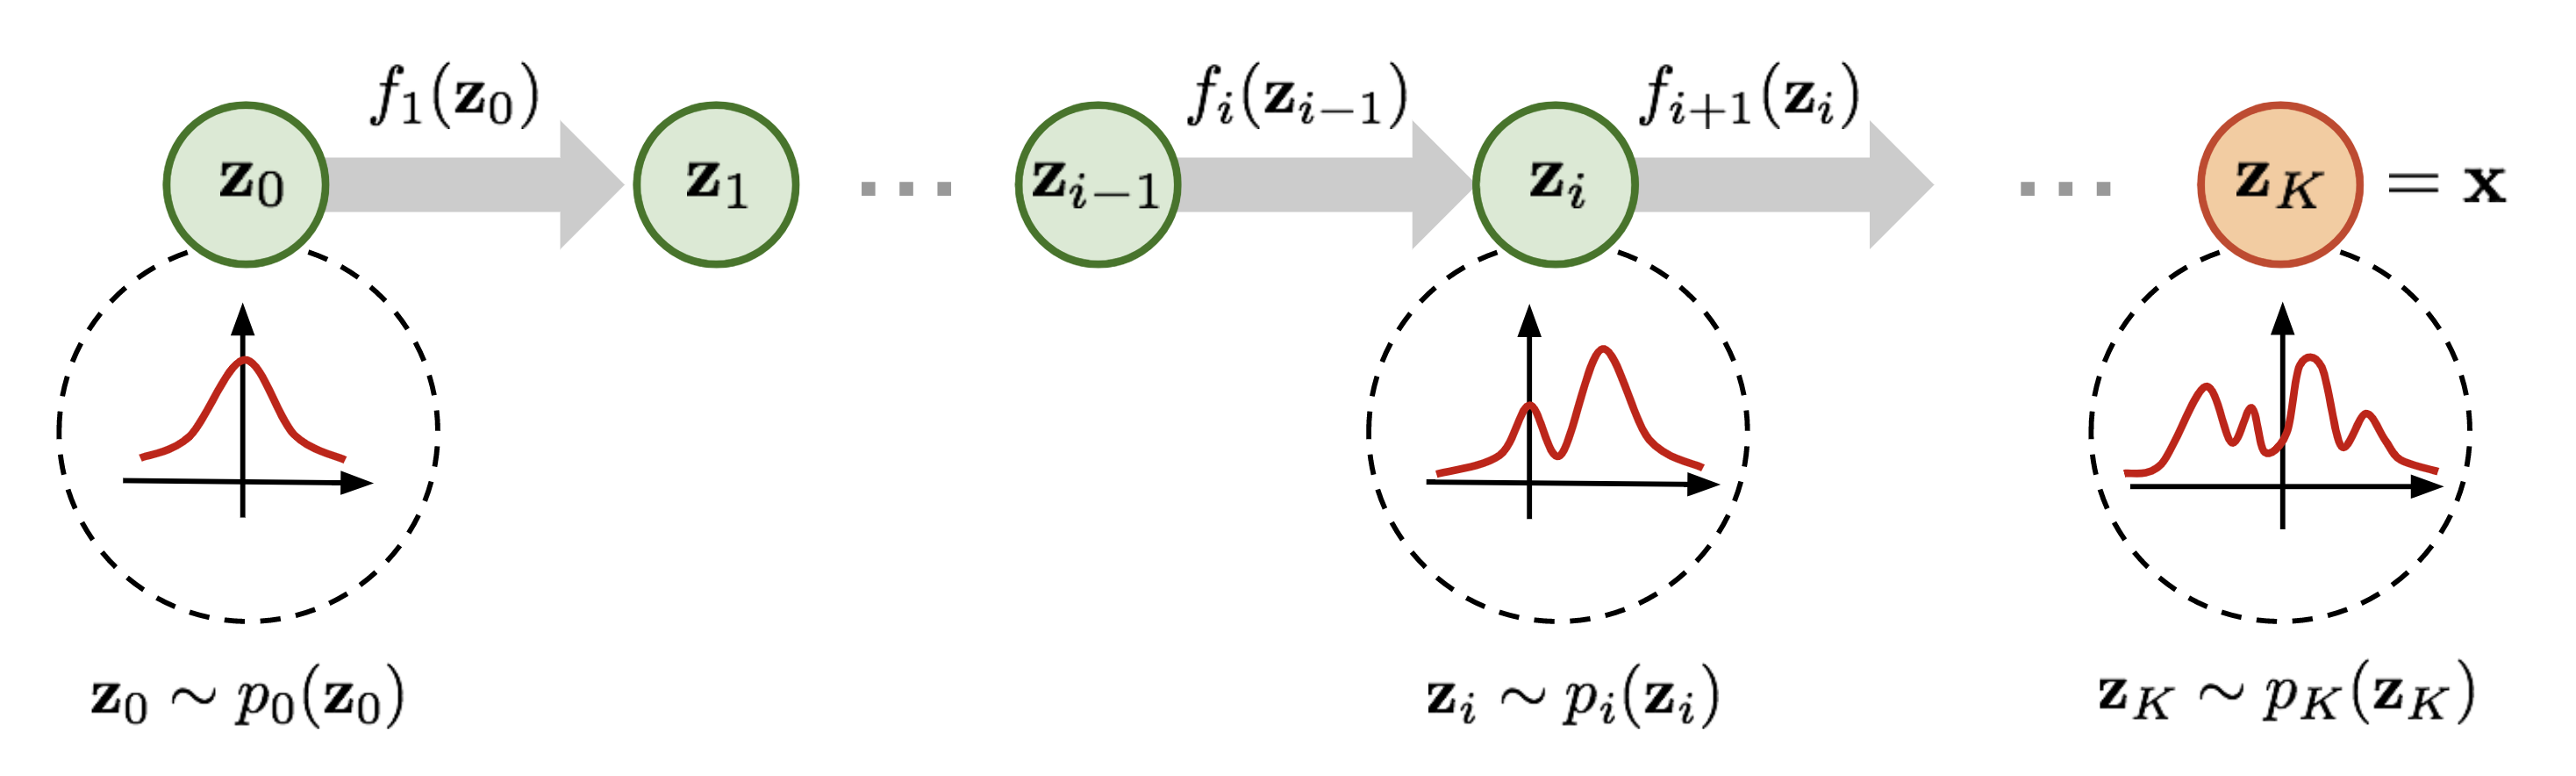
\includegraphics[width=0.95\linewidth]{figs/normalizing-flow}
	\end{figure}
	\vspace{-0.4cm}
	\[
		\log \pt(\bx) = \log p(\bff_K \circ \dots \circ \bff_1(\bx)) + \sum_{k=1}^K\log \left|\det \left(\frac{\partial \bff_k}{\partial \bff_{k-1}}\right)\right|.
	\]
	\vspace{-0.4cm}
\end{frame}
%=======
\begin{frame}{Towards Continuous-Time Normalizing Flows}
	\myfootnotewithlink{https://arxiv.org/abs/1906.02735}{Chen R. T. Q. et al. Residual Flows for Invertible Generative Modeling, 2019}
	Up to this point, we have considered discrete-time normalizing flows:
	\vspace{-0.3cm}
	\[
		\bx_{t+1} = \bff_{\btheta}(\bx_t, t); \quad \log p(\bx_{t+1}) = \log p(\bx_{t}) - \log \left| \det \frac{\partial \bff_{\btheta}(\bx_t)}{\partial \bx_{t}} \right| .
	\]
	\vspace{-0.3cm}
	\eqpause
	\begin{block}{Residual Flows}
		Let's consider the flow $\bff_{\btheta}(\bx, t) = \bx + \bv_{\btheta}(\bx, t)$:
		\[
			\bx_{t+1} = \bff_{\btheta}(\bx_t, t) = \bx_t + \bv_{\btheta}(\bx_t, t)
		\]
		\eqpause
		\vspace{-0.5cm}
		\begin{itemize}
			\item This transformation is invertible by the Banach fixed point theorem if $\bv_{\btheta}$ is contractive, i.e. with Lipschitz constant $<1$.
			\item Here $\bff_{\btheta}$ is the NF \textbf{bijection}, $\bv_{\btheta}$ is the \textbf{velocity} (vector field).
			\item The update $\bx_{t+1} - \bx_t = \bv_{\btheta}(\bx_t, t)$ is a \textbf{finite-difference} approximation of a derivative.
		\end{itemize}
	\end{block}
\end{frame}
%=======
\begin{frame}{Towards Continuous-Time Normalizing Flows}
	Residual dynamics $\bx_{t+1} = \bx_t + \bv_{\btheta}(\bx_t, t)$ is an Euler step with $h=1$:
	\[
		\frac{\bx(t + h) - \bx(t)}{h} = \bv_{\btheta}(\bx(t), t)
	\]
	\eqpause
	Taking the limit $h \rightarrow 0$, we obtain continuous-time dynamics.
	\begin{block}{Continuous-Time Dynamics}
		Consider an Ordinary Differential Equation (ODE):
		\vspace{-0.3cm}
		\begin{align*}
		   \frac{d \bx(t)}{dt} &= \bv_{\btheta}(\bx(t), t); \quad \text{with initial condition }\bx(t_0) = \bx_0. \\
		   \nextonslide{
		   \bx(t_1) &= \int^{t_1}_{t_0} \bv_{\btheta}(\bx(t), t) d t  + \bx_0
		   }
		\end{align*}
		\vspace{-0.6cm}
	\end{block}
	Here, $\bv_{\btheta}: \bbR^m \times [t_0, t_1] \rightarrow \bbR^m$ is a \textbf{velocity vector field}.
\end{frame}
%=======
\begin{frame}{Ordinary Differential Equations (ODEs)}
	\begin{align*}
		\frac{d \bx(t)}{dt} &= \bv_{\btheta}(\bx(t), t); \quad \text{with initial condition }\bx(t_0) = \bx_0. \\
		\bx(t_1) &= \int^{t_1}_{t_0} \bv_{\btheta}(\bx(t), t) d t  + \bx_0
	\end{align*}
	\vspace{-0.6cm}
	\eqpause
	\begin{block}{Flow}
		Let call \textbf{the flow} $\bpsi: \bbR^m \times [t_0, t_1] \rightarrow \bbR^m$ the solution of ODE:
		\[
			\frac{d \bpsi_t(\bx_0)}{dt} = \bv_{\btheta}(\bpsi_t(\bx_0), t); \quad \text{with initial condition }\bpsi_0(\bx_0) = \bx_0.
		\]
	\end{block}
	\eqpause
	\begin{block}{Numerical Solution of ODEs}
		\vspace{-0.5cm}
		\[
			\bpsi_t(\bx_0) = \int^{t}_{t_0} \bv_{\btheta}(\bx(s), s) d s  + \bx_0 \nextonslide{\approx {\color{teal}\ODESolve_v(\bx_0, \btheta, t_0, t)}.}
		\]
		\eqpause
		Here, we require the numerical routine $\ODESolve_v(\bx_0, \btheta, t_0, t)$.
	\end{block}
\end{frame}
%=======
\begin{frame}{Numerical Solution of ODEs}
	\myfootnotewithlink{https://en.wikipedia.org/wiki/Heun's\_method}{Image credit: https://en.wikipedia.org/wiki/Heun's\_method}   
	\[
		\bpsi_t(\bx_0) = \int^{t}_{t_0} \bv_{\btheta}(\bx(s), s) d s  + \bx_0 \nextonslide{\approx {\color{teal}\ODESolve_v(\bx_0, \btheta, t_0, t)}.}
	\]
	$\ODESolve_v(\bx_0, \btheta, t_0, t)$ consists of sequence of iterative update steps.
	\eqpause
	\begin{block}{Euler Update Step}
		\begin{minipage}[t]{0.5\columnwidth}
			\vspace{-0.3cm}
			\[
	  			\frac{\bx(t + h) - \bx(t)}{h} = \bv_{\btheta}(\bx(t), t)
			\]
			\[
	  			\bx(t + h) = \bx(t) + h \cdot \bv_{\btheta}(\bx(t), t)
			\]
		\end{minipage}%
		\eqpause
		\begin{minipage}[t]{0.5\columnwidth}
			\vspace{-0.8cm}
			\begin{figure}
				\centering
				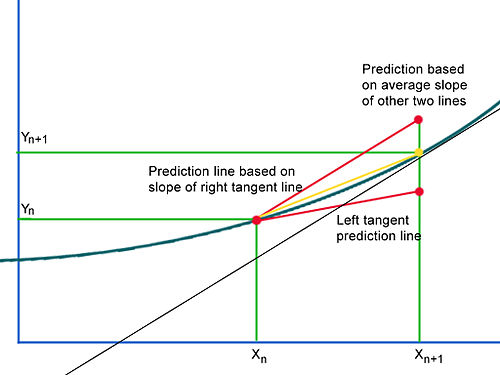
\includegraphics[width=\linewidth]{figs/heun_method}
			\end{figure}
		\end{minipage}
	\end{block}
	\vspace{-1.0cm}
	\begin{block}{Heun's Update Step}
		\vspace{-0.3cm}
		\[
			\bx'(t + h) = \bx(t) + h \cdot \bv_{\btheta}(\bx(t), t)
		\]
		\[
			\bx(t + h) = \bx(t) + \frac{h}{2} \cdot \left(\bv_{\btheta}(\bx(t), t) + \bv_{\btheta}(\bx'(t+h), t + h)\right)
		\]
	\end{block}
\end{frame}
%=======
\begin{frame}{Generative Models Taxonomy}
	\renderTaxonomy{ode}
\end{frame}
%=======
\begin{frame}{Continuous-Time Normalizing Flows: Neural ODE}
	\myfootnotewithlink{https://arxiv.org/abs/1806.07366}{Chen R. T. Q. et al. Neural Ordinary Differential Equations, 2018}   
	\begin{block}{Neural ODE}
		\vspace{-0.2cm}
		\[
  			\frac{d \bx(t)}{dt} = \bv_{\btheta}(\bx(t), t); \quad \text{with initial condition }\bx(t_0) = \bx_0
		\]
		\vspace{-0.3cm}
	\end{block}	
	\eqpause
	\begin{block}{Euler \ODESolve}
		\vspace{-0.3cm}
		\[
		    \bx(t + h) = \bx(t) + h \cdot \bv_{\btheta}(\bx(t), t)
		\]
		\vspace{-0.5cm}
	\end{block}
	\eqpause
	\begin{itemize}
		\item Consider $[t_0, t_1] = [0, 1]$ for simplicity.
		\item If $\bx(0)$ is a random variable with density~$p_0(\bx)$,
		\item Then, for any $t$, $\bx(t)$ is a random variable with density $p_t(\bx)$.
	\end{itemize}
\end{frame}
%=======
\begin{frame}{Continuous-Time Normalizing Flows: Intuition}
	\myfootnotewithlink{https://arxiv.org/abs/1810.01367}{Grathwohl W. et al. FFJORD: Free-form Continuous Dynamics for Scalable Reversible Generative Models, 2018}  
	\[
 		\frac{d \bx(t)}{dt} = \bv_{\btheta}(\bx(t), t); \quad \text{with initial condition }\bx(t_0) = \bx_0
	\]
	\eqpause
	\vspace{-0.5cm}
	\begin{itemize}
		\item $p_t(\bx) = p(\bx, t)$ describes the \textbf{probability path} interpolating between $p_0(\bx)$ and $p_1(\bx)$.
		\item {\color{gray}What is the difference between $p_t(\bx(t))$ and $p_t(\bx)$?}
	\end{itemize}
	\eqpause
	\begin{figure}
		\centering
		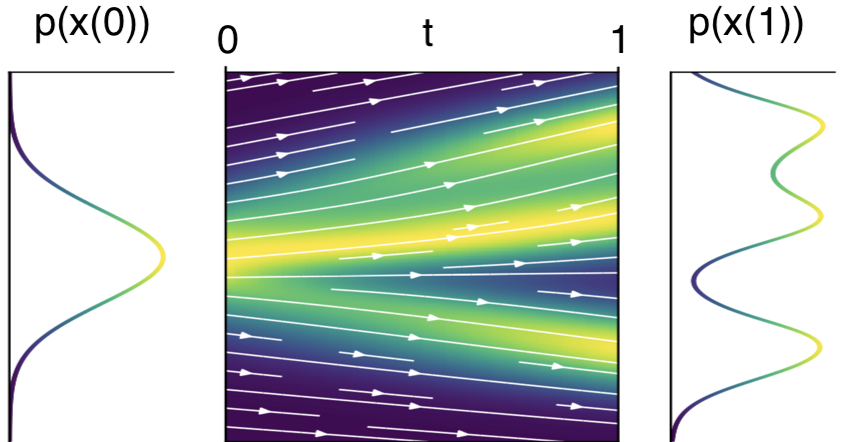
\includegraphics[width=0.75\linewidth]{figs/cnf_flow.png}
	\end{figure}
\end{frame}
%=======
\begin{frame}{Continuous-Time Normalizing Flows: Reversibility}
	\myfootnotewithlink{https://arxiv.org/abs/1806.07366}{Chen R. T. Q. et al. Neural Ordinary Differential Equations, 2018}   
	\begin{block}{Theorem (Picard)}
		If $\bv$ is continuously differentiable with a bounded derivative in $\bx$ and continuous in $t$, then the ODE has a \textbf{unique solution} given by a flow $\bpsi_t$.
	\end{block}
	\eqpause
	This guarantees the ODE is \textbf{uniquely reversible}. 
	\vspace{-0.3cm}
	\begin{align*}
		\bpsi_1(\bx_0) &= \bx_0 + \int_{0}^{1} \bv_{\btheta}(\bpsi_t(\bx_0), t) dt \\
		\bx(1) &= \bx(0) + \int_{0}^{1} \bv_{\btheta}(\bx(t), t) dt \\
		\bx(0) &= \bx(1) + \int_{1}^{0} \bv_{\btheta}(\bx(t), t) dt
	\end{align*}
	\eqpause
	\textbf{Note:} Unlike discrete-time flows, $\bv$ need not be invertible (uniqueness ensures bijection).
	\eqpause
	How can we compute $p_t(\bx)$ at arbitrary $t$?
\end{frame}
%=======
\section{Continuity Equation for CNF Log-Likelihood}
%=======
\begin{frame}{Continuous-Time NF}
	\myfootnotewithlink{https://arxiv.org/abs/1806.07366}{Chen R. T. Q. et al. Neural Ordinary Differential Equations, 2018}   
	\begin{block}{Theorem (Continuity Equation)}
		If $\bv$ is continuously differentiable in $\bx$ (with bounded derivative) and continuous in $t$, and $p_t(\bx) > 0$, then
		\[
			\frac{d \log p_t(\bx(t))}{d t} = - \tr \left( \frac{\partial \bv(\bx(t), t)}{\partial \bx(t)} \right)
		\]
		\vspace{-0.3cm}
	\end{block}
	\eqpause
	This result states: given $\bx_0 = \bx(0)$, the solution to the continuity equation gives the density $p_1(\bx(1))$.
	\begin{block}{Solution}
		\vspace{-0.3cm}
		\[
			\log p_1(\bx(1)) = \log p_0(\bx(0)) - {\color{teal}\int_{0}^{1} \tr  \left( \frac{\partial \bv(\bx(t), t)}{\partial \bx(t)} \right) dt}.
		\]
		\vspace{-0.3cm}
	\end{block}
	\eqpause
	\begin{itemize}
		\item This provides the density \textbf{along the trajectory}.
		\item However, {\color{teal}the latter term} is difficult to estimate efficiently.
	\end{itemize}
\end{frame}
%=======
\section{SDE Basics}
%=======
\begin{frame}{Stochastic Differential Equation (SDE)}
	\myfootnotewithlink{https://arxiv.org/abs/2506.02070}{Holderrieth P., Erives E. An Introduction to Flow Matching and Diffusion Models, 2025}
	\vspace{-0.3cm}
	\begin{block}{Wiener Process}
		$\bw(t)$ is the standard Wiener process (Brownian motion), defined~by:
		\vspace{-0.3cm}
		\begin{minipage}{0.5\columnwidth}
			\begin{enumerate}
				\item $\bw(0) = 0$ (almost surely);
				\item $\bw(t)$ has independent increments;
				\item $\bw(t)$ trajectories are continuous;
				\item $\bw(t) - \bw(s) \sim \cN(0, (t-s) \bI)$ for $t>s$;
			\end{enumerate}
		\end{minipage}%
		\begin{minipage}{0.45\columnwidth}
			\centering
			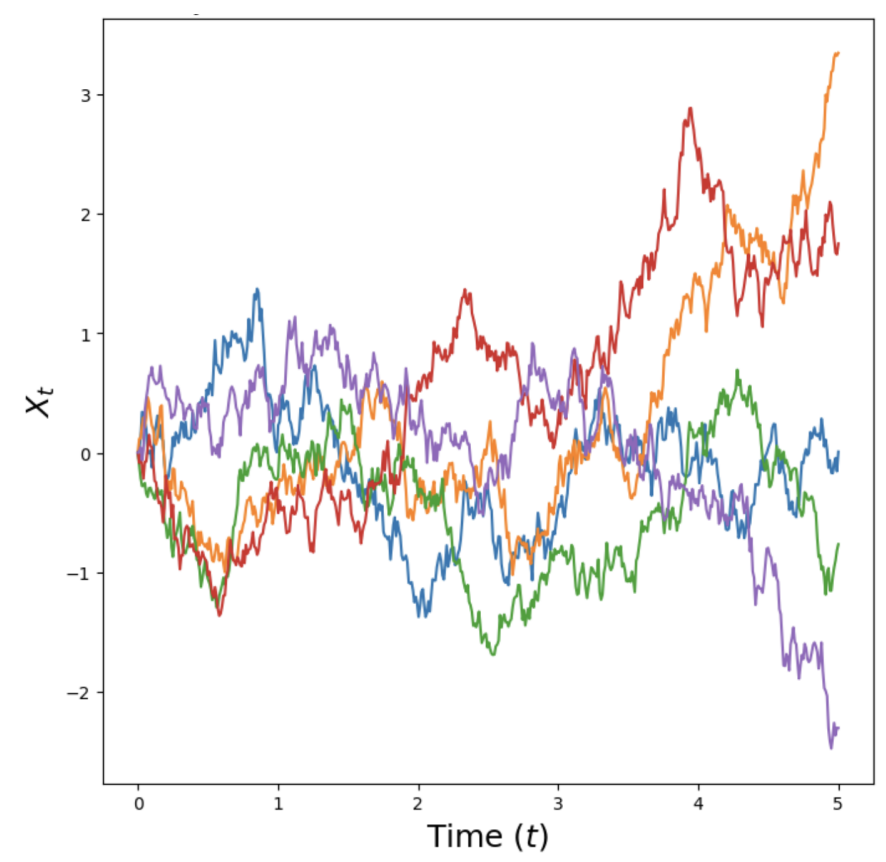
\includegraphics[width=\linewidth]{figs/brownian_motion}
		\end{minipage}
	\end{block}
	\vspace{0.3cm}
	\eqpause
	$d\bw = \bw(t+dt) - \bw(t) = \cN(0, \bI \cdot dt ) = \bepsilon \cdot \sqrt{dt}$, where $\bepsilon \sim \cN(0, \bI)$.
\end{frame}
%=======
\begin{frame}{Stochastic Differential Equation (SDE)}
	\[
 		\frac{d \bx}{dt} = \bv(\bx, t) \Rightarrow d\bx = \bv(\bx, t) dt
	\]
	\eqpause
	Let's define a stochastic process $\bx(t)$ with initial condition $\bx(0) \sim p_0(\bx) = \pd(\bx)$:
	\[
		d\bx = \bff(\bx, t) dt + {\color{violet}g(t) d \bw}
	\]
	\eqpause
	\vspace{-0.5cm}
	\begin{itemize}
		 \item $\bff(\bx, t): \bbR^m \times [0, 1] \rightarrow \bbR^m$ is the \textbf{drift} term (vector field).
		 \item $g(t): \bbR \rightarrow \bbR$ is the \textbf{diffusion} term (if $g(t)=0$, we recover the standard ODE).
		 \item $\bw(t)$ is the standard Wiener process ($d\bw = \bepsilon \cdot \sqrt{dt}$).
		 \item We do not have the flow $\bpsi_t(\bx_0)$ notion anymore, since trajectories are stochastic.
	\end{itemize}
\end{frame}
%=======
\begin{frame}{It\^{o} Integration Basics}
	\myfootnotewithlink{https://arxiv.org/abs/2510.21890}{Lai C. et al. The Principles of Diffusion Models, 2025}
	The SDE should be understood in its \textbf{integral form} (It\^{o} sense):
	\[
		\bx(t) = \bx(0) + {\color{violet}\int_0^t \bff(\bx(s), s) \, ds} + {\color{teal}\int_0^t g(s) \, d\bw(s)}
	\]
	\eqpause
	\vspace{-0.5cm}
	\begin{itemize}
		\item {\color{violet}The first integral} is a classical (Riemann) integral.
		\item {\color{teal}The second integral} is an \textbf{It\^{o} stochastic integral}.
	\end{itemize}
	\eqpause
	\[
		\int_0^t g(s) \, d\bw(s) = \lim_{N \to \infty} \sum_{i=0}^{N-1} g(t_i) \bigl(\bw(t_{i+1}) - \bw(t_i)\bigr)
	\]
	\vspace{-0.3cm}
	\begin{itemize}
		\item Brownian paths are continuous but a.s. \textbf{nowhere differentiable} $\Rightarrow$ Fundamental Theorem of Calculus fails.
		\item Instead, SDEs require \textbf{It\^{o} calculus} (e.g., It\^{o}'s lemma).
		\item Expressions $d\bx$, $dt$, $d\bw$ are \textbf{formal shorthand} for infinitesimal increments.
	\end{itemize}
\end{frame}
%=======
\begin{frame}{Stochastic Differential Equation (SDE)}
	\[
		d\bx = \bff(\bx, t) dt + g(t) d \bw
	\]
	\begin{block}{Theorem}
		If $\bff$ is continuously differentiable with a bounded derivative in $\bx$ 
		and continuous in $t$ and $g(t)$ is continuous then the SDE has the solution given by unique process $\bx(t)$.
	\end{block}
	\eqpause
	\begin{itemize}
		\item Unlike ODEs, the initial condition $\bx(0)$ doesn't uniquely determine the trajectory.
		\item There are two sources of randomness: 
		\begin{itemize}
			\item the initial distribution $p_0(\bx)$;
			\item the Wiener process $\bw(t)$.
		\end{itemize}
	\end{itemize}
\end{frame}
%=======
\begin{frame}{Stochastic Differential Equation (SDE)}
	\[
		d\bx = \bff(\bx, t) dt + g(t) d \bw
	\]
	\vspace{-0.3cm}
	\begin{block}{Discretizing the SDE (Euler-Maruyama Update) – \SDESolve}
		\vspace{-0.3cm}
		\[
			{\color{violet}\bx(t + dt) = \bx(t) + \bff(\bx(t), t) \cdot dt} + {\color{teal}g(t) \cdot \bepsilon \cdot \sqrt{dt}}
		\]
		\eqpause
		If $dt=1$, then
		\vspace{-0.3cm}
		\[
			{\color{violet}\bx_{t + 1} = \bx_t + \bff(\bx_t, t)} + {\color{teal}g(t) \cdot \bepsilon}
		\]
		\vspace{-0.7cm}
	\end{block}
	\eqpause
	\begin{itemize}
		\item At any time $t$, the process has density $p_t(\bx) = p(\bx, t)$.
		\item $p: \bbR^m \times [0,1] \rightarrow \bbR_+$ specifies a \textbf{probability path} from $p_0(\bx)$ to $p_1(\bx)$.
		\item How can we obtain the probability path $p_t(\bx)$ for $\bx(t)$?
	\end{itemize}
\end{frame}
%=======
\begin{frame}{Stochastic Differential Equation (SDE)}
	\vspace{-0.4cm}
	\[
		d\bx = \bff(\bx, t) dt + g(t) d \bw,\quad d \bw = \bepsilon \cdot \sqrt{dt},\quad \bepsilon \sim \cN(0, \bI).
	\]
	\vspace{-0.4cm}
	\begin{block}{Theorem (Kolmogorov-Fokker-Planck)}
		If $p_t(\bx) \in C^{1,2}$ (i.e., $C^1$ in $t$ and $C^2$ in $\bx$), then
		\vspace{-0.2cm}
		\[
			\frac{\partial p_t(\bx)}{\partial t} = - \diver\left(\bff(\bx, t) p_t(\bx)\right) + \frac{1}{2}g^2(t) \Delta_{\bx}p_t(\bx)
		\]
		\eqpause
		Here,
		\[
			\diver (\bv) = \sum_{i=1}^m \frac{\partial v_i(\bx)}{\partial x_i} = \tr\left( \frac{\partial \bv(\bx)}{\partial \bx}  \right)
		\]
		\[
			\Delta_{\bx}p_t(\bx) = \sum_{i=1}^m \frac{\partial^2 p_t(\bx)}{\partial x_i^2} = \tr\left( \frac{\partial^2 p_t(\bx)}{\partial \bx^2}  \right)
		\]
		\eqpause
		\[
			\frac{\partial p_t(\bx)}{\partial t} = \tr\left( - \frac{\partial}{\partial \bx} \bigl[ \bff(\bx, t) p_t(\bx)\bigr] + \frac{1}{2} g^2(t) \frac{\partial^2 p_t(\bx)}{\partial \bx^2} \right)
		\]
	\end{block}
\end{frame}
%=======
\begin{frame}{Stochastic Differential Equation (SDE)}
	\begin{block}{Theorem (Kolmogorov-Fokker-Planck)}
		\vspace{-0.2cm}
		\[
			\frac{\partial p_t(\bx)}{\partial t} = \tr\left( - \frac{\partial}{\partial \bx} \bigl[ \bff(\bx, t) p_t(\bx)\bigr] + \frac{1}{2} g^2(t) \frac{\partial^2 p_t(\bx)}{\partial \bx^2}\right)
		\]
		\vspace{-0.2cm}
	\end{block}
	\begin{itemize}
		\item The KFP theorem is a necessary and sufficient condition (it uniquely defines $p_t(\bx)$).
		\item This generalizes the continuity equation for continuous-time NF:
		\[
			\frac{d \log p_t(\bx(t))}{d t} = - \tr \left( \frac{\partial \bv(\bx(t), t)}{\partial \bx(t)} \right).
		\]
	\end{itemize}
	\eqpause
	\begin{block}{Special Case: constant density $p_t(\bx)$}
		Let's find the SDE for which $p_t(\bx) = \text{const}$ (i.e., if $\bx(0) \sim p_0(\bx)$, then $\bx(t) \sim p_0(\bx)$.).
		\eqpause
		\[
			\frac{\partial p_t(\bx)}{\partial t} = 0 \quad \Leftrightarrow \quad \tr\left( - \frac{\partial}{\partial \bx} \bigl[ \bff(\bx, t) p_t(\bx)\bigr] + \frac{1}{2} g^2(t) \frac{\partial^2 p_t(\bx)}{\partial \bx^2}\right) = 0
		\]
	\end{block}
\end{frame}
%=======
\begin{frame}{Langevin SDE (Special Case)}
	\[
		\frac{\partial p_t(\bx)}{\partial t} = 0 \quad \Leftrightarrow \quad \tr\left( - \frac{\partial}{\partial \bx} \bigl[ \bff(\bx, t) p_t(\bx)\bigr] + \frac{1}{2} g^2(t) \frac{\partial^2 p_t(\bx)}{\partial \bx^2}\right) = 0
	\]
	\vspace{-0.3cm}
	\eqpause
	\[
		\frac{\partial}{\partial \bx} \bigl[ \bff(\bx, t) p_t(\bx)\bigr] = \frac{1}{2} g^2(t) \frac{\partial^2 p_t(\bx)}{\partial \bx^2}
	\]
	\eqpause
	\[
		\bff(\bx, t) p_t(\bx) = \frac{1}{2} g^2(t) \frac{\partial p_t(\bx)}{\partial \bx}
	\]
	\eqpause
	\[
		\bff(\bx, t) = \frac{1}{2} g^2(t) \frac{1}{p_t(\bx)}\frac{\partial p_t(\bx)}{\partial \bx} = \frac{1}{2} g^2(t) \frac{\partial}{\partial \bx} \log p_t(\bx)
	\]
	\eqpause
	Let ${\color{olive}g(t)=1}$, then ${\color{violet}\bff(\bx, t) = \frac{1}{2} \frac{\partial}{\partial \bx} \log p_t(\bx)}$.
	\[
		d \bx = {\color{violet}\frac{1}{2} \frac{\partial}{\partial \bx} \log p_t(\bx) d t} + {\color{olive}1} \cdot d \bw
	\]
\end{frame}
%=======
\begin{frame}{Langevin SDE (Special Case)}
	\myfootnotewithlink{https://www.stats.ox.ac.uk/~teh/research/compstats/WelTeh2011a.pdf}{Welling M. Bayesian Learning via Stochastic Gradient Langevin Dynamics, 2011}
	Let's find the SDE for which $p_t(\bx) = \text{const}$ (i.e., if $\bx(0) \sim p_0(\bx)$, then $\bx(t) \sim p_0(\bx)$.).
	\[
		d \bx = {\color{violet}\frac{1}{2} \frac{\partial}{\partial \bx} \log p_t(\bx) d t} + {\color{olive}1} \cdot d \bw
	\]
	\eqpause
	\begin{block}{Discretized Langevin SDE}
		\vspace{-0.3cm}
		\[
			\bx_{t + 1} - \bx_t = \frac{\eta}{2} \cdot \frac{\partial}{\partial \bx} \log p_t(\bx) + \sqrt{\eta} \cdot \bepsilon, \quad \eta \approx dt.
		\]
		\vspace{-0.4cm}
	\end{block}
	\eqpause
	Setting the stationary density to the model distribution, $p_t(\bx) = \pt(\bx)$ for all $t$:
	\begin{block}{Langevin Dynamic}
		\vspace{-0.3cm}
		\[
			\bx_{t + 1} = \bx_t + \frac{\eta}{2} \cdot \nabla_{\bx} \log \pt(\bx) + \sqrt{\eta} \cdot \bepsilon, \quad \eta \approx dt.
		\]
		\vspace{-0.3cm}
	\end{block}
	We (partially) explained, why Langevin dynamics is working.
\end{frame}
%=======
\begin{frame}{Summary}
	\begin{itemize}
		\item Continuous-time normalizing flows leverage neural ODEs to define continuous-time trajectories $\bx(t)$, relaxing many constraints of discrete-time flows.
		\vfill
		\item If $\bx_0$ is a random variable, this yields a \textbf{probability path} $p_t(\bx)$ as time evolves. The continuity equation describes the evolution of $\log p(\bx, t)$ over time.
		\vfill
		\item An SDE defines a stochastic process with drift and diffusion terms; ODEs are a special case of SDEs.
		\vfill
		\item The KFP equation describes the probability dynamics of an SDE.
		\vfill
		\item The Langevin SDE preserves a constant probability path.
	\end{itemize}
\end{frame}
%=======
\end{document}